\section{Automatic Differentiation}
In the following, we will consider a \say{set} of data points
\begin{equation*}
    X\in\R^{N\times d}
\end{equation*}
made of $N$ inputs of size $d$, and targets
\begin{equation*}
    Y\in\Y^n
\end{equation*}
where $\Y$ is an arbitrary set. It can be for instance $\Y=\R$ is the case of regression, a finite set such as $\iset{1}{C}$ in the case of classification, or $\Y=\R^{d'}$ in a more general setup.

\subsection{Introduction}
As stated previously, neural networks is a very expressive class of functions. However, the associated optimization problem is in general non-convex, giving very few theoretical guarantees and no closed-form expression. In practice, this is not an issue, since such optimization problem can be solved using \emph{gradient descent}.
\subsubsection{Loss function}

Gradient descent is done by minimizing the average of a differentiable loss function $\L:\Y\times\Y\to\R$. For instance, for regression, we might choose the squared error:
\begin{equation*}
    \L(\hat{y}, y) = (\hat{y}-y)^2
\end{equation*}
For classification, we might choose the logistic loss. Its expression for a two-classes model (that is $y\in\{0, 1\}$) is:
\begin{equation*}
    \L(\hat{y}, y) = y\log\hat{y} + (1-y)\log(1-\hat{y})
\end{equation*}
More generally, for a $C$-classes model (that is $y\in\iset{1}{C}$), the cross-entropy loss is:
\begin{equation*}
    \L(\hat{y}, y) =  \sum_{c=1}^C y_c \log \hat{y}_c
\end{equation*}
The average of the loss function is then given by:
\begin{equation*}
    J(f) = \frac{1}{N}\sum_{n=1}^N \L\left(f(X_n), Y_n\right)
\end{equation*}
which we will try to minimize.

\subsubsection{Gradient descent}
The idea behind gradient descent is therefore to be able to compute the gradient of $\L$ with respect to the paramters $\theta$ for each point of the dataset:
\begin{figure}[H]
    \centering 
    \begin{minipage}{0.4\textwidth}
    \begin{minted}[escapeinside=||, mathescape=true]{python}
for epoch in range(EPOCHS):
    for x, y in zip(X, Y):
        compute |$\nabla_\theta\L$|
        |$\theta = \theta - \gamma\nabla_\theta\L$|
    \end{minted}
    \end{minipage}
    \caption{Pseudo-code of gradient descent}
\end{figure}
The only remaining challenge is the computation of $\nabla_\theta\L$, preferably automatically; this is the problem which we will address in this chapter.

\subsection{Optimization methods}
\subsubsection{Stochastic Gradient Descent}
\subsubsection{Batch gradient descent}
\subsubsection{Minibatch gradient descent}
\subsubsection{Newton's method}

\subsection{Computing gradients}
\subsubsection{By hand}
The most straightforward approach to computing $\nabla_\theta\L$ would be to derive it on paper. Nevertheless, this is complicated, as it involves very long computations using matrix calculus.

Furthermore, this approach is not modular, as changing the loss function or adding a layer requires to re-derive the gradient from scratch. Such a method does not scale: if the computations can be done in a reasonable amount of time for small models using linear and activation layers, complex models introduced in the next chapters have enormous gradient expressions, making the computation way too long and tidious to be done by hand.

\subsubsection{Numerical differentiation}
A first automatic approach to compute the gradient automatically would be to use \emph{numerical differentiation}, a method to estimate the derivative of the function using finite differences. Recall that since the derivative of a real-valued function is the limit of its growth rate:
\begin{equation*}
    f'(x) = \lim_{h\to0} \frac{f(x+h)-f(x)}{h}
\end{equation*}
one can approximate the derivative using the slope between two points close to $x$:
\begin{equation*}
    f'(x) \simeq \frac{f(x+h)-f(x)}{h}
\end{equation*}
for some small number $h$. However, this approach does not work well in practice because of round-off errors which can have a strong impact on the result and cause gradient descent to diverge.

\subsubsection{Symbolic differentiation}
To avoid round-off errors, another approach could be to use symbolic differentiation: the idea is to formally compute the expression of the derivative and then to evaluate it numerically. The issue with symbolic differentiation is its scalability: without optimization of the computation, it can produce exponentially large expressions that take a long time to symbolically compute and numerically evaluate. To maintain reasonable expression sizes, one needs to apply simplification operations between each step, resulting in a heavy computational cost.

Hopefully, we do not need all the expressivity that symbolic differentiation has: we are only interested in the numerical evaluation of the derivative; we do not need to keep the formal expression, only the numerical evaluation. 

This is the idea of \emph{automatic differentiation} with accumulation: we will keep the idea of symbolic differentiation by computing the derivative as an operation level, but reduce the size of intermediate computations by only keeping the numerical values.

\subsection{Automatic differentiation}
\subsubsection{Computational Graphs}
Automatic differentiation uses a data structure called \emph{Computational Graphs} to represent the computation that is happening inside the model.
\begin{figure}[H]
    \centering
    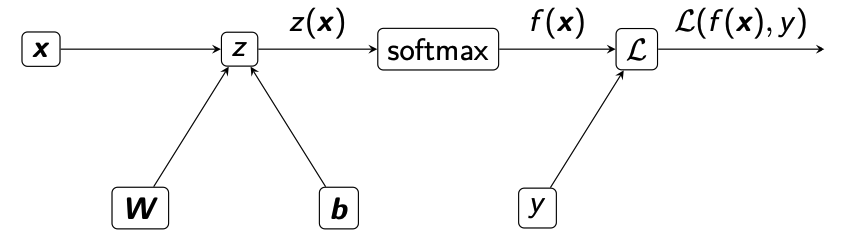
\includegraphics[width=.7\textwidth]{autodiff/computational-graph.png}
    \caption{Computational graph for $\L(\softmax(Wx+b), y)$}
    \label{fig:computational-graph}
\end{figure}
In Figure \ref{fig:computational-graph}, reading from left to right, we can see that the weights $W$, the biases $b$ and the input $x$ are combined to create a function $z(x)$; to the result of this operation is applied $\softmax$, creating $f(x)$. Finally, $f(x)$ is combined with $y$ using the loss function $\L$, giving the final result of the computation, $\L(f(x), y)$.

Computational graphs can then be used to apply the main algorithm to compute the gradient, called \emph{backpropagation}. We will illustrate its behavior by considering the function $f(x, y, z) = (x+y)\times z$, to which is associated the following computational graph:
\begin{figure}[H]
    \centering
    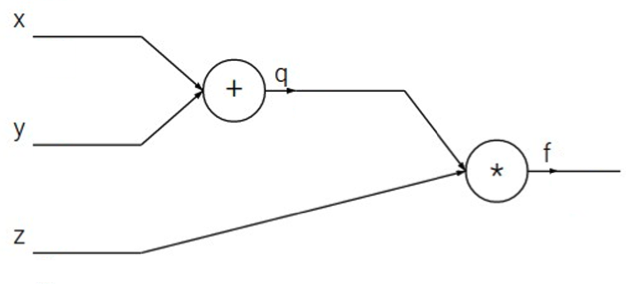
\includegraphics[width=.5\textwidth]{autodiff/simple-graph.png}
    \caption{Computational graph for $f(x, y, z) = (x+y)\times z$}
\end{figure}

\subsubsection{Forward pass}
The first step of backpropagation is to compute the outputs during a \emph{forward pass}. This is simply done by replacing each input by its numerical value, and applying the operations described by the nodes of the graph. Using $x=-2$, $y=5$, $z=-4$ in the previous example yields:
\begin{figure}[H]
    \centering
    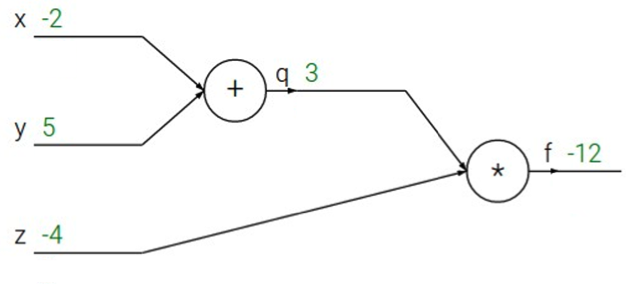
\includegraphics[width=.5\textwidth]{autodiff/forward-graph.png}
    \caption{Forward pass}
\end{figure}

\subsubsection{Backward pass}
The backward pass allows us to compute the derivatives, in our case $\partfrac{f}{x}$, $\partfrac{f}{y}$ and $\partfrac{f}{z}$. Instead of computing the value at each node from left to right (forward pass), we will compute the values of the derivatives from right to left, starting from the output (backward pass).

\begin{itemize}
    \item Starting from the output node, we have that $\partfrac{f}{f}=1$.
    \item Going backward to the $z$ input node, we have that $\partfrac{f}{z}=q$, since $f=qz$. We can then use the results of the forward pass to find the value of $q$, and deduce $\partfrac{f}{z}=3$.
    \item Similarly, $\partfrac{f}{q}=z=-4$.
    \item Going further back into the graph, we aim at computing $\partfrac{f}{y}$. Using chain rule, we know that:
    \begin{equation*}
        \partfrac{f}{y}=\partfrac{q}{y}\partfrac{f}{q}
    \end{equation*}
    This equation can be interpreted in terms of \say{gradient stream}: we want to compute the \emph{downstream gradient} $\partfrac{f}{y}$, that is the gradient \say{after the node}. This gradient can therefore be expressed using the chain rule as the product of the \emph{local gradient} $\partfrac{q}{y}$ and the \emph{upstream gradient} $\partfrac{f}{q}$, that is the gradient computed at the previous node.
    \begin{equation*}
        \underbrace{\partfrac{f}{y}}_{\textnormal{Downstream}}=\underbrace{\partfrac{q}{y}}_{\textnormal{Local}} \underbrace{\partfrac{f}{q}}_{\textnormal{Upstream}}
    \end{equation*}
    Like in previous cases, we can compute the local gradient $\partfrac{q}{y}=1$ since $q=x+y$. The upstream gradient is also known at this point of the pass, due to the backward direction, hence $\partfrac{f}{y}=1\times-4=-4$
    \item The same approach using the chain rule can be used for $\partfrac{f}{x}=\partfrac{q}{x}\partfrac{f}{q}=1\times -4=-4$.
\end{itemize}

\subsubsection{Modularity}
A benefit of backpropagation is its modularity: the gradient computation can be broke down into the computation of the downstream gradient knowing the upstream gradient and the local gradient of the node. 

Consider for instance a function $f$ taking $x$ and $y$ as inputs, and producing an output $z$. This function is a node somewhere in a possibly very complex computational graph, but we do not need the whole information about the rest of the computation: to compute the downstream gradient, we only need local information, that is upstream and local gradients. 

We are given the upstream gradient of the loss that we want to compute with respect to our output, $\partfrac{\L}{z}$. Our goal is now simply to propagate the gradient computation by providing the downstream derivatives, that is $\partfrac{\L}{x}$ and $\partfrac{\L}{y}$. Since we know the expression of $f$, we are able to compute the local derivatives $\partfrac{z}{x}$ and $\partfrac{z}{y}$; using chain rule, we can therefore provide the downstream gradient.
\begin{figure}[H]
    \centering
    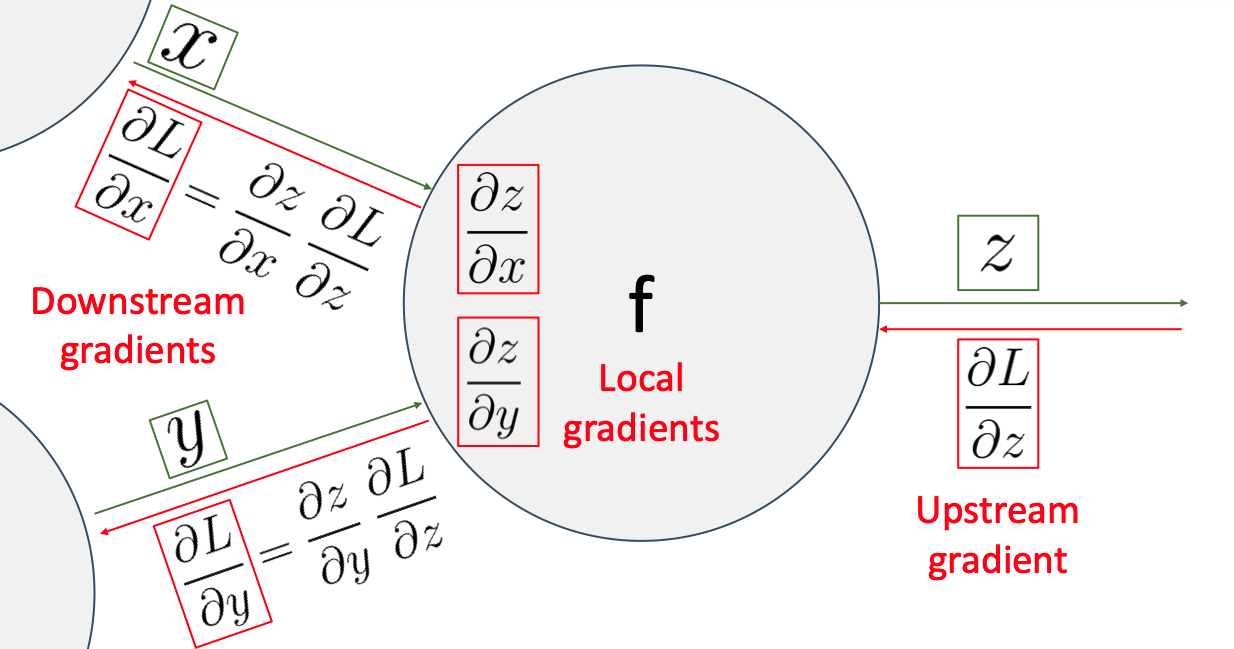
\includegraphics[width=.6\textwidth]{autodiff/modularity.png}
    \caption{Local process of computing the downstream gradient}
\end{figure}

\subsubsection{A complete example}
\begin{figure}[H]
    \centering
    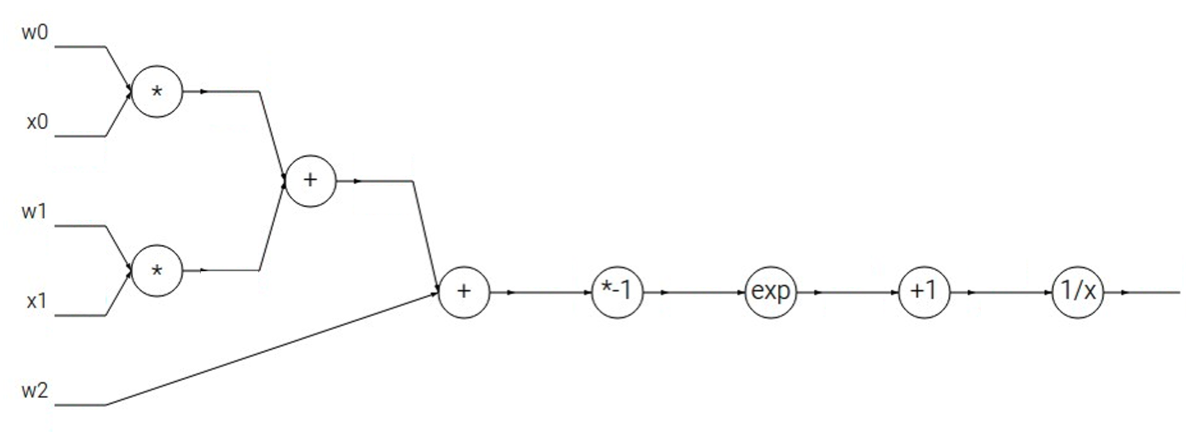
\includegraphics[width=.6\textwidth]{autodiff/complete-example.png}
    \caption{Computational graph for the function $f(x, w) = \frac{1}{1+e^{-(w_0x_0+w_1x_1+w_2)}}$}
\end{figure}
We do not have to break down the gradient computation only into elementary operations such as additions or multiplications: we can define blocks, such as \say{Sigmoid}, and hard-code their gradients to avoid using automatic differentiation on it.

\subsection{Extension to multivariate calculus}
So far, we only considered backpropagation in the case of scalars. The same principle can nevertheless be extended to multivariate calculus using vectors and matrices.

\subsubsection{Reminder on vector derivatives}
For a real-valued function $f:\R\longrightarrow\R$, the regular derivative is a scalar:
\begin{equation*}
    \frac{\dd f}{\dd x} = \partfrac{f}{x} \in \R
\end{equation*}

For a function taking a vector and returning a scalar, that is $f:\R^n\longrightarrow\R$, its derivative is its \emph{gradient}, that is:
\begin{equation*}
    \nabla f\in\R^n \where \left(\nabla f\right)_i = \partfrac{f}{x_i}
\end{equation*}
The $i$-coordinate of the gradient is the partial derivative of $f$ with respect to the $i$-th variable of the input vector.

Finally, for a differentiable function taking a vector and returning another vector, that is $f:\R^n\longrightarrow\R^m$, its derivative is its \emph{Jacobian}, that is:
\begin{equation*}
    J_f 
    = \begin{bmatrix} \partfrac{f}{x_1} & \dots & \partfrac{f}{x_n}\end{bmatrix} 
    = \begin{bmatrix} 
        \nabla^\tp f_1\\ 
        \vdots\\ 
        \nabla^\tp f_m
    \end{bmatrix}
    = \begin{bmatrix}
        \partfrac{f_1}{x_1} & \dots & \partfrac{f_1}{x_n}\\
        \vdots & \ddots & \vdots\\
        \partfrac{f_m}{x_1} & \dots & \partfrac{f_m}{x_n}
    \end{bmatrix}
    \in\mathscr{M}_{m, n}(\R)
\end{equation*}

\subsubsection{Example: linear layer gradient}
Consider a linear layer of the form $f(x)=Wx$ where $W$ is an $m\times n$ matrix. The $i$-th coordinate of the output of is
\begin{equation*}
    f_i = W_ix=\sum_j W_{i,j}x_j
\end{equation*}
where $W_i$ is the $i$-th row of $W$. Therefore, its Jacobian is:
\begin{equation*}
    (J_f)_{i, j} = \partfrac{f_i}{x_j} = W_{i, j}
\end{equation*}
hence $J_f=W$.

\subsubsection{Generalized multivariate chain rule}
Consider two differentiable functions $f:\R^m\longrightarrow\R^k$ and $g:\R^n\longrightarrow\R^m$, and $a\in\R^n$. The chain rule is expressed as:
\begin{equation}
    D_a(f\circ g) = D_{g(a)}f\circ D_ag
\end{equation}
where $D_af$ for instance is the derivative of $f$ evaluated in $a$. Furthermore, the Jacobians verify:
\begin{equation}
    J_{f\circ g}(a)=J_f(g(a)) J_g(a)
\end{equation}